%%%%%%%%%%%%%%%%%%%%%%%%%%%%%%%%%%%%%%%%%%%%%%%%%%%%%%%%%
%Este documento representa la plantilla de los articulos%
%a ser editados para la revista, realizada bajo codigo  %
%        Latex, con una clase ``article``               %   
%          PUBLICACIONES EN CIENCIAS                    %               
%                Y  TECNOLOGIA.                         %
%        Realizado por Adriana Araujo                   %
%       Revisado por Hugo Lara              (2014)      %        
%              Cuerpo editorial.                        %
%%%%%%%%%%%%%%%%%%%%%%%%%%%%%%%%%%%%%%%%%%%%%%%%%%%%%%%%%
\documentclass[11pt,twoside,A5]{article}
\usepackage[spanish]{babel}
\usepackage[utf8]{inputenc}
\usepackage{amsmath}
\usepackage{amsfonts}
\usepackage{amssymb}
\usepackage{amscd}
\usepackage{psfrag}
\usepackage{graphicx}
\usepackage{url}
\usepackage{listings}
\usepackage[ruled,vlined,spanish,onelanguage]{algorithm2e}
\usepackage{float}
\lstset{ frame=Ltb,
framerule=0pt,
aboveskip=0.5cm,
framextopmargin=3pt,
framexbottommargin=3pt,
framexleftmargin=0.1cm,
%xleftmargin=0.5cm,
framesep=0pt,
rulesep=.4pt,
backgroundcolor=\color{gray97},
rulesepcolor=\color{black},
%
stringstyle=\ttfamily,
showstringspaces = false,
basicstyle=\footnotesize\ttfamily,
commentstyle=\color{gray45},
keywordstyle=\bfseries,
%
numbers=left,
%numbersep=0.2cm,
numberstyle=\tiny,
numberfirstline = false,
breaklines=true
}
\usepackage[font=footnotesize,labelfont=bf]{caption}
\usepackage{subcaption}
\usepackage[T1]{fontenc}
\usepackage{color}
\definecolor{gray97}{gray}{.97}
\definecolor{gray75}{gray}{.75}
\definecolor{gray45}{gray}{.45}
%%%%%%%%%%%%%%%%%%%%%%%%%%%%%%%%%%
%\theoremstyle{theorem}
\newtheorem{thm}{Theorem}[section]
\newtheorem{prop}{Proposition}[section]
\newtheorem{clly}{Corollary}[section]
\newtheorem{lem}{Lemma}[section]
\newtheorem{pf}{Proof}[section]
%\theoremstyle{definition}
\newtheorem{defi}{Definition}[section]
\newtheorem{exam}{Example}[section]
\newtheorem{rk}{Remark}[section]
\def\proof{\mbox {\it Proof.~}}
\newcommand{\en}{\~n}
\newcommand{\figura}{\stepcounter{figure}}
\newcommand{\cuadro}{\stepcounter{table}}
\renewcommand{\tablename}{Tabla}
\newtheorem{pot}{Proof of Theorem} %\ref{mainthm}}
\renewcommand{\lstlistingname}{Listado}
%%%%%%%%%%%%%%%%%%%%%%%%%%%%%%%%%%%%%%%%%%
\def\N{\mathbb{N}}
\def\Z{\mathbb{Z}}
\def\Q{\mathbb{Q}}
\def\R{\mathbb{R}}
\def\C{\mathbb{C}}
\def\K{\mathbb{K}}
\def\V{\mathbb{V}}
\def\U{\mathbb{U}}
\def\O{\mathcal{O}}
\def\A{\mathcal{A}}
\def\L{\mathcal{L}}
\def\Rc{\mathcal{R}}
\newcommand{\vect}{\overrightarrow}
\newcommand{\modN}{\;\text{(mod $N$)}}

\usepackage[pass,paperwidth=15cm,paperheight=22cm]{geometry}
\paperheight=22cm
  \paperwidth=15cm
\setlength{\oddsidemargin}{-0.5cm} \setlength{\evensidemargin}{-1.0cm}
\setlength{\topmargin}{-1.5cm} \setlength{\textwidth}{11.5cm}
\setlength{\textheight}{17.5cm}

\setcounter{page}{1}
%%%%%%%%%%%%%%%%%%%%%%%%%%%%%%%%%%

\newcommand{\reflistings}[1]{Listado \ref{#1}}
\newcommand{\refplistings}[1]{(\reflistings{#1})}

\newcommand{\reffigure}[1]{Figura \ref{#1}}
\newcommand{\refpfigure}[1]{(\reffigure{#1})}

\newcommand{\reftable}[1]{Cuadro \ref{#1}}
\newcommand{\refptable}[1]{(\reftable{#1})}

\newcommand{\refalgorithm}[1]{Algoritmo \ref{#1}}
\newcommand{\refpalgorithm}[1]{(\refalgorithm{#1})}

\newcommand{\quotes}[1]{``#1''}

\newcommand{\sourcecode}[2][\footnotesize]{{\ttfamily#1#2}}

\newcommand{\link}[1]{{\footnotesize\url{#1}}}

%%%%%%%%%%%%%%%%%%%%%%%%%%%%%%%%%%%%%%%
\usepackage{fancyhdr}
\pagestyle{fancy}
%%%%%%%%%%%%%%%%%%%%%%%%%%%%%%%%%%%%%%%%%%%%%%%%%%%%%%%%%%%%%%%%%%%%%%%%%%%%%%%%%%%%%%%%%%%%%%%%%%%%%%%%%%%%%%%
%%%%%%%%SECCION DEL TITULO Y TIRILLA BIBLIOGRAFICA(ESTA ULTIMA PARA USO INTERNO DEL CUERPO EDITORIAL)%%%%%%%%%%
%%%%%%%%%%%%%%%%%%%%%%%%%%%%%%%%%%%%%%%%%%%%%%%%%%%%%%%%%%%%%%%%%%%%%%%%%%%%%%%%%%%%%%%%%%%%%%%%%%%%%%%%%%%%%%%
\begin{document}
\title{
\vspace{-1.1in}
\begin{flushleft}
{\normalsize \begin{center}
%{\em\bf Publicaciones en Ciencias y Tecnolog\'ia}\\ 
%\scriptsize{Vol 7, N$^{0}$2, Jul--Dic 2013, pp.7--15,   ISSN:1856-8890, Dep\'osito Legal:pp200702LA2730 }
%\small{Art\'iculo en revisi\'on.  ISSN:1856-8890, Dep\'osito Legal: pp200702LA2730}
\end{center}}
\end{flushleft}
\hrule \vspace{0.5in}{ARQUITECTURA HÍBRIDA DE NAVEGACIÓN PARA ROBOT PIONEER PD3X} }
%%%%%%%%%%%%%%%%%%%%%%%%%%%%%%%%%%%%%%%%%%%%%%%%%%%%%%%%%%%%%%%%%%%%%%%%%%%%%%%%%%%%%%%%%%%%%%%%%%%%%%%%%%%%%%%
%%%%%%%%SECCION AUTORES Y FILIACION DE LOS MISMOS %%%%%%%%%%%%%%%%%%%%%%%%%%%%%%%%%%%%%%%%%%%%%%%%%%%%%%%%%%%%%%
%%%%%%%%%%%%%%%%%%%%%%%%%%%%%%%%%%%%%%%%%%%%%%%%%%%%%%%%%%%%%%%%%%%%%%%%%%%%%%%%%%%%%%%%%%%%%%%%%%%%%%%%%%%%%%%

\author{ 
\footnote{  {\it\scriptsize  Decanato de Ciencias y Tecnolog\'ia,} 
{\it\scriptsize Universidad Centroccidental Lisandro Alvarado,}
{\it\scriptsize Barquisimeto, Venezuela, thejorgemylio@gmail.com}
}\hspace{1mm}{Jorge Parra}
 \hspace{3mm} 
\footnote{  {\it\scriptsize  Decanato de Ciencias y Tecnolog\'ia,} 
{\it\scriptsize Universidad Centroccidental Lisandro Alvarado,}
{\it\scriptsize Barquisimeto, Venezuela, sauljabin@gmail.com}
}\hspace{1mm}{ Saúl Piña} \\
 %\hspace{3mm} 
%\footnote{  {\it\scriptsize Departamento-Instituto-Facultad}, 
%{\it\scriptsize Universidad-Instituci\'on (filiaci\'on)},
%{\it\scriptsize Lugar, Pa\'is, email}
%}\hspace{5mm}{ Nombre autor 3 }
% \hspace{3mm} 
%\hspace{3mm}
%\footnote{ {\it\scriptsize  Departamento de Ingenier\'ia Industrial,  Instituto Tecnol\'ogico de Celaya}, 
%{\it\scriptsize Instituto Tecnol\'ogico de Celaya},  
%{\it\scriptsize M\'exico, gesparza@itc.mx }
%}\hspace{5mm} { Luis Gerardo Esparza-D\'iaz}
}

%\vspace{-15mm}
\date{\small{Octubre 2014}
}

%\date{}
%%%%%%%%%%%%%%%%%%%%%%%%%%%%%%%%%%
\maketitle 
%%%%%%%%%%%%%%%%%%%%%%%%%%%%%%%%%%%%%%%%%%%%%%%%%%%%%%%%%%%%%%%%%%%%%%%%%%
% SECCION TITULO CORTO E INICIALES AUTORES, HASTA DOS AUTORES:
% APELLIDO 1, INICIAL NOMBRE 1. ; APELLIDO 2, INICIAL NOMBRE 2.
%                        MAS DE DOS 
%                APELLIDO, INICIAL NOMBRE. et al
%%%%%%%%%%%%%%%%%%%%%%%%%%%%%%%%%%%%%%%%%%%%%%%%%%%%%%%%%%%%%%%%%%%%%%%%%%%
\fancyhead{} \fancyhead[CE]{{\scriptsize ARQUITECTURA HÍBRIDA DE NAVEGACIÓN PARA ROBOT PIONEER PD3X}}
\fancyhead[CO]{ Jorge Parra, Saúl Piña
}
\fancyfoot{}
%\fancyfoot[CO,CE]{\scriptsize{{Publicaciones en Ciencias y Tecnolog\'ia.} Vol 7,N$^{0}$2, Jul--Dic 2013, pp.07--15.}}
%\fancyfoot[CO,CE]{Publicaciones en Ciencias y Tecnolog\'ia. Art\'iculo en revisi\'on}
\fancyfoot[RO,LE]{\thepage}

%%%%%%%%%%%%%%%%%%%%%%%%%%%%%%%%%%%%%%%%%%%%%%%%%%%%%%%%%%%%%%%%%%%%%%%%%%%%%
%%%%%%%%%%%%%%%%%%SECCION DE RESUMEN Y ABSTRACT%%%%%%%%%%%%%%%%%%%%%%%%%%%%%%
%%%%%%%%%%%%%%%%%%%%%%%%%%%%%%%%%%%%%%%%%%%%%%%%%%%%%%%%%%%%%%%%%%%%%%%%%%%%%
\begin{center}
{\bf\small Resumen}
%\vspace{-5mm}

\vspace{-3mm} \hspace{.05in}\parbox{4.5in} {{\small %\footnotesize 

En el presente informe se da a conocer de manera detallada el diseño, desarrollo e implementación 
de la arquitectura de navegación híbrida AuRA para el robot Pionner P3DX, 
con el objetivo de planificar rutas entre dos puntos cualesquiera en un ambiente conocido.
La arquitectura construye el camino más corto aplicando el Algoritmo de Dijkstra sobre el diagrama de Voronoi asociado
al entorno. Se segmentó el espacio a través de la Triangulación de Delaunay.
Por otra parte, se explica el funcionamiento e instalación sobre sistemas operativos Windows o Linux de la aplicación de software 
desarrollada. Se exponen los resultados y conclusiones del conjunto de pruebas 
realizadas para validar la arquitectura. En los resultados alcanzados se encontró 
que el robot tiene la capacidad de dirigirse por el espacio efectivamente más no completamente eficiente. 
También se pudo observar que el robot responde satisfactoriamente a obstaculos inesperados. 

 \textbf{Palabras clave}: Robótica, ARIA, AuRA, Arquitectura Híbrida, Pioneer P3DX.}}
\end{center}
\pagebreak


%\begin{center}
%{\bf\small T\'ITULO EN INGL\'ES \\ Abstract}
%
%\vspace{-3mm} \hspace{.05in}\parbox{4.5in} {{\small %\footnotesize 
%
%Cuerpo del abstract  
%
%     \textbf{Keywords}:  kw 1, kw 2, ... .}}
%\end{center}
%%%%%%%%%%%%%%%%%%%%%%%%%%%%%%%%%%%%%%%%%%%%%%%%%%%%%%%%%%%%%%%%%%%%%%%%%%%%%%%%%%%%%%%
%                           CUERPO DEL ARTICULO
%%%%%%%%%%%%%%%%%%%%%%%%%%%%%%%%%%%%%%%%%%%%%%%%%%%%%%%%%%%%%%%%%%%%%%%%%%%%%%%%%%%%%%%
%\pagebreak

\section*{Introducción}

La robótica móvil es un campo de investigación que supone la integración de numerosas disciplinas
entre las que resaltan la electrónica, ingeniería mecánica,
inteligencia artificial, estadística, entre otros. Tiene como objetivo 
guiar el curso de un robot movil sobre un entorno con obstculos conocido o desconocido,
a través de un sistema que integra la percepción del entorno mediante
sensores, toma de decisiones y acciones.

Las tareas involucradas en la navegación de un robot móvil son: la percepción del
entorno, la planificación de una trayectoria libre de obstáculos, y la conducción del vehiculo a través de la referencia establecida.
Es necesario que se incluya la capacidad de reaccionar ante situaciones inesperadas.

La arquitectura AuRA propone un enfoque de control donde se fusiona los paradigmas deliberativo y reactivo,
integra todas las tareas expuestas anteriormente, por ende, le permitirá al robot movil responder a eventos inesperados, desenvolverse en 
entornos no estructurados y a la vez cumplir con los objetivos de la misión. La implementancion de esta arqitectura supone un conocimiento previo
del entorno, el cual servira como insumo para la planificación global de la misión.

En el presente trabajo se expone todo el proceso de implementación de la arquitectura híbrida AuRA sobre el robot movil P3DX,
con un razonador espacial principalmente basada en el diagrama de Voronoi y en el algoritmo voraz Dijkstra para el calculo de 
la ruta óptima.

\section*{Pioneer P3DX}

El Pionner P3DX \refpfigure{fig:pioneer} es un robot ligero ideal para ser usado en el interior de laboratorios o aulas de clases. El robot cuenta con una rueda y un motor ubicados a cada lado del mismo. Además, tiene una rueda en la parte posterior que le ayuda a mantener el equilibrio.
Igualmente, el Pionner P3DX posee sensores de ultrasonido o sonares, empleados para detectar obstáculos en el ambiente.
Es uno de los robots más popularmente usados en las áreas de la educación e investigación. Puedes ser fácilmente personalizado y mejorado, integrandolo con accesorios de diversa índole. Por otra parte, posee un conjunto completo de aplicaciones y librerías que sustentan el desarrollo de proyectos de investigación.

\begin{figure}[here]
	\centering
	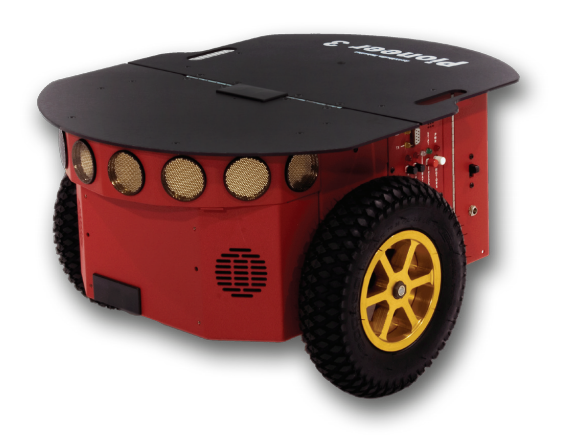
\includegraphics[width=6cm]{pioneer.png} 
	\caption{Robot Pioneer P3DX.}
	\label{fig:pioneer}
\end{figure} 

\begin{figure}[here]
	\centering
	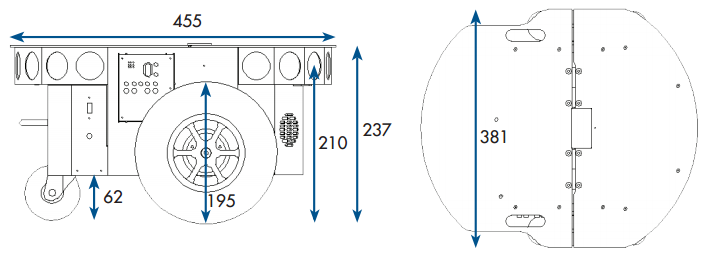
\includegraphics[width=8cm]{pioneer-dimensiones.png} 
	\caption{Dimensiones en milímetros del robot Pioneer P3DX.}
	\label{fig:pioneer-dimensiones}
\end{figure} 

\subsubsection*{Especificaciones del Pioneer P3DX}

\noindent\textbf{Construcción}
\\
\indent\textbf{Dimensiones:} 45,5 cm de largo por 38,1 cm de ancho \refpfigure{fig:pioneer-dimensiones}.
\\
\indent\textbf{Cuerpo:} 1,6 mm de aluminio.
\\
\indent\textbf{Neumáticos:} de caucho relleno de goma.
\\\\
\noindent\textbf{Operación}
\\
\indent\textbf{Peso del Robot:} 9 kg.
\\
\indent\textbf{Carga operativa:} 17 kg.
\\\\
\noindent\textbf{Potencia}
\\
\indent\textbf{Tiempo de ejecución:} 8-10 horas con 3 baterías.
\\
\indent\textbf{Tiempo de carga:} 12 horas o 2,4 horas.
\\
\indent\textbf{Baterías:} Soporta hasta 3 a la vez.
\\
\indent\textbf{Tensión:} 12 V.
\\
\indent\textbf{Capacidad:} 7,2 Ah.



\section*{Arquitectura AuRA}

La arquitectura AuRA \cite{arkin1997} (Autonomous Robot Architecture) introducida por Ronald Arkin, plantea un enfoque híbrido
de navegación para robots móviles. Está constituida principalmente por dos capas, una deliberativa basada en la inteligencia artificial
tradicional y otra reactiva basada en teoría de esquemas. En la \reffigure{fig:aura} se puede observar la representación del AuRA, 
la capa deliberativa la componen el \textit{planificador de misión}, \textit{razonador espacial} y el \textit{secuenciador del plan}. En el nivel más alto se encuentra el \textit{planificador de misión}, representa la interfaz con el humano y permite establecer los objetivos, 
las restricciones y los parámetros en los que debe operar el robot. El \textit{razonador espacial} puede ser referido como navegador, este usa la información cartográfica
almacenada para construir la ruta deseada que el robot debe seguir para completar la misión. El \textit{secuenciador del plan}
puede ser comparado con un piloto, convierte la ruta generada por el \textit{razonador espacial} al conjunto de comportamientos (esquemas) que debe ejecutar la capa reactiva. En la capa reactiva, el \textit{control de esquema} es el responsable de llevar a cabo y monitorear en tiempo real el conjunto de comportamientos que el secuenciador ordena ejecutar, cada comportamiento esta asociado a un esquema perceptual, en otras palabras, cada estimulo genera una respuesta. 

\begin{figure}[here]
\begin{center}
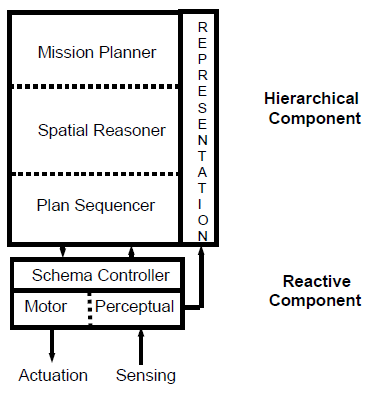
\includegraphics[width=5cm]{aura.png} 
\caption{Representación de arquitectura AuRA.}
\label{fig:aura}
\end{center}
\end{figure} 

\subsubsection*{Fortalezas de la Arquitectura AuRA}

Modularidad, flexibilidad, generalización e hibridación, son los características resaltantes de esta arquitectura.

\textbf{Modularidad}, es altamente modular debido a su diseño en capas, lo que permite intercambiar o mejorar
los componentes sin afectar el funcionamiento general.

\textbf{Flexibilidad}, esta arquitectura permite integrar diferentes modelos de inteligencia artificial 
para la construcción de rutas, aprendizaje y adaptación. 

\textbf{Generalización}, puede ser empleado en distintos dominios como la manufactura, navegación, entre otros.

\textbf{Hibridación}, fusiona los paradigmas deliberativo y reactivo, lo que le permite al robot interactuar con eventos inesperados mientras intenta satisfacer sus metas.

\section*{Entorno de Desarrollo}

Para llevar a cabo la presente investigación se desarrollo una aplicación cliente
con las siguientes herramientas de software:

\textbf{ARIA} (Advanced Robot Interface for Applications) \cite{aria2014},
es una librería desarrollada en el lenguaje de programación C++ para todas las
plataformas MobileRobots/ActivMedia. Provee el conjunto de herramientas necesarias
para controlar y monitorear de forma dinámica al robot y sus elementos. Ademas, esta librería
incluye implementaciones llamadas \textit{wrapper} en los lenguajes de programación Python y Java, siendo este último 
el lenguaje de desarrollo para este investigación.

\textbf{MobileSim} \cite{mobilesim2014}, es un software para la simulación de plataformas
MobileRobots/ActivMedia. Permite usar la librería ARIA y sus wrappers. Es un ambiente
ideal para realizar experimentación y pruebas de los algoritmos desarrollados antes de
implementarlos en los robots reales.
 
\textbf{Eclipse IDE} \cite{eclipse2014}, es un entorno de desarrollo integrado para múltiples lenguajes de 
programación en los que destacan Java y C++. Provee las herramientas necesarias para el desarrollo, depuración  
y compilación de aplicaciones.

\textbf{Java} \cite{java2014}, es un lenguaje de programación de propósito general, orientado a objetos y de alto nivel. 
 
\section*{Configuración del Entorno}

Antes de configurar el entorno de desarrollo es necesario descargar el código fuente del proyecto,
este está disponible al público con licencia de software \textbf{MIT} en la siguiente dirección:
\\ \link{https://bitbucket.org/sauljabin/ariajava-p3dx}.

\subsubsection*{Requisitos}
\begin{enumerate}
\item Sistema operativo de 32bits.
\item Java 7 o mayor.
\item Eclipse 4 o mayor.
\end{enumerate}

\subsubsection*{Configuración del Entorno Sobre Windows}

\begin{enumerate}
\item Instalar \sourcecode{MobileSim-0.7.2-1.exe}, disponible en: \\ \link{http://robots.mobilerobots.com/wiki/MobileSim}.
\item Instalar \sourcecode{ARIA-2.7.6.exe}, disponible en: \\ \link{http://robots.mobilerobots.com/wiki/ARIA}.
\item Agregar a la variable de entorno \sourcecode{PATH} la ruta: \\ \sourcecode{C:\textbackslash Program Files\textbackslash MobileRobots\textbackslash ARIA\textbackslash bin\textbackslash}.
\item Dirigirse a la ruta \sourcecode{C:\textbackslash Program Files\textbackslash MobileRobots\textbackslash ARIA\textbackslash bin\textbackslash}, cambiar el nombre del archivo
\sourcecode{AriaVC10.dll} a  \sourcecode{Aria.dll}.
\item Importar proyecto a eclipse.
\item Agregar al \sourcecode{Java Build Path} el wrapper Java de ARIA que se encuentra en la ruta: \\ \sourcecode{C:\textbackslash Program Files\textbackslash MobileRobots\textbackslash ARIA\textbackslash java\textbackslash Aria.jar}.
\item Verificar que la variable  \sourcecode{PATH\_LIBARIA} del archivo  \sourcecode{CONFIG.props} 
	  sea igual a:  \sourcecode{C\textbackslash:\textbackslash\textbackslash Program Files\textbackslash\textbackslash MobileRobots\textbackslash\textbackslash ARIA\textbackslash\textbackslash bin\textbackslash\textbackslash }.
\end{enumerate}

\subsubsection*{Configuración del Entorno Sobre Debian/Ubuntu}

\begin{enumerate}
\item Descargar el archivo \sourcecode{MobileSim-0.7.3+gcc4.6.tgz}, disponible en: \\ \link{http://robots.mobilerobots.com/wiki/MobileSim}.
\item Ejecutar los siguientes comandos por consola para instalar MobileSim:
\sourcecode{ 
\\ \$ tar xzvf MobileSim-0.7.3+gcc4.6.tgz
\\ \# mv -f MobileSim-0.7.3 /usr/local/MobileSim
\\ \# ln -s -f /usr/local/MobileSim/MobileSim /usr/bin/mobilesim}
\item Descargar el archivo \sourcecode{ARIA-2.8.1+gcc4.6.tgz}, disponible en: \\ \link{http://robots.mobilerobots.com/wiki/ARIA}.
\item Ejecutar los siguientes comandos por consola para instalar ARIA:
\sourcecode{
\\ \$ tar xzvf ARIA-2.8.1+gcc4.6.tgz
\\ \# mv -f Aria-2.8.1 /usr/local/Aria
\\ \# echo '/usr/local/Aria/lib' > /etc/ld.so.conf.d/aria.conf
\\ \# ldconfig}
\item Importar proyecto a eclipse.
\item Agregar al \sourcecode{Java Build Path} el wrapper Java de ARIA que se encuentra en la ruta: \sourcecode{/usr/local/Aria/java/Aria.jar}
\item Verificar que la variable \sourcecode{PATH\_LIBARIA} del archivo \sourcecode{CONFIG.props} 
	  sea igual a: \sourcecode{/usr/local/Aria/lib/}
\end{enumerate}

\section*{Implementación de la Arquitectura}

\subsection*{Capa Deliberativa}

\subsubsection*{\textit{Planificador de misión}}

Con el fin de planificar la misión, se desarrolló una interfaz gráfica intuitiva que permite configurar
los parámetros generales, cargar la información cartográfica y además presentar la ruta óptima que deberá recorrer el robot \refpfigure{fig:planificador}. 

\begin{figure}[here]
\begin{center}
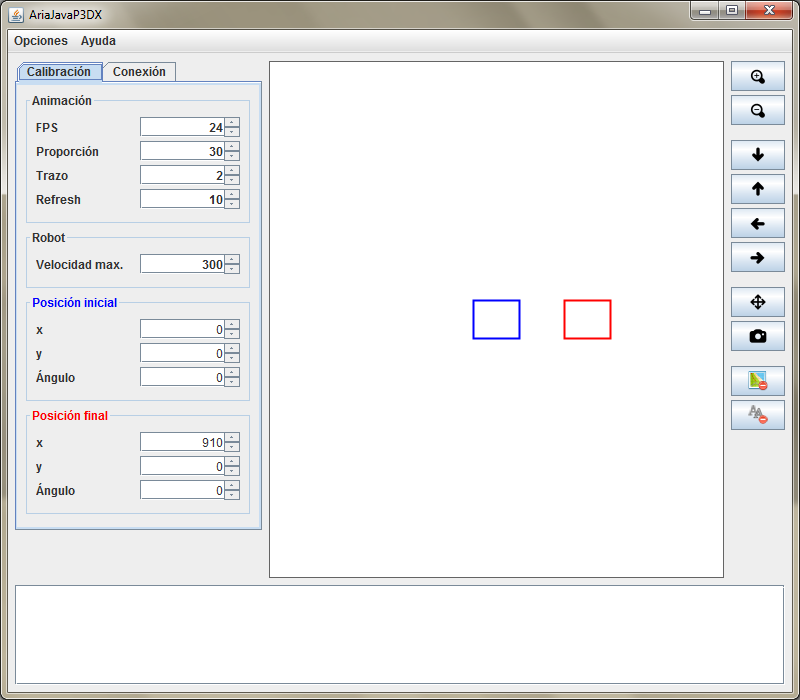
\includegraphics[width=10cm]{ventana-principal.png} 
\caption{Planificador de misión.}
\label{fig:planificador}
\end{center}
\end{figure} 

Por otra parte es posible cargar mapas a través de archivos de texto plano con extensión \textit{.map}, 
este formato de archivo es compatible con MobileSim y puede ser generado o editado por
Mapper3 \cite{mapper2014}.

En el \reflistings{lst:map} se puede apreciar un ejemplo de como está estructurado un archivo \textit{.map},
cabe destacar que en este formato las longitudes son medidas en milímetros.

\begin{minipage}{\linewidth}
\begin{lstlisting}[caption={Ejemplo archivo mapa.}, label=lst:map]
2D-Map
Cairn: RobotHome -5000 -5000 0 "" ICON "Home"
Cairn: Goal 5000 5000 0 "" ICON "Goal" 
LineMinPos: -6000 -6000
LineMaxPos: 6000 6000
NumLines: 4
LINES
-6000 6000 6000 6000
-6000 -6000 6000 -6000
-6000 6000 -6000 -6000
6000 6000 6000 -6000
\end{lstlisting}
\end{minipage}

A continuación se describen las líneas que conforman el mapa:

\noindent\textbf{Línea 1:} \sourcecode{2D-Map}, indica el tipo de mapa.
\\\textbf{Línea 2:} \sourcecode{Cairn: RobotHome -5000 -5000 0 \textquotedbl\textquotedbl~ICON \textquotedbl Home\textquotedbl}, representa la posición inicial del robot.
\\\textbf{Línea 3:} \sourcecode{Cairn: Goal 5000 5000 0 \textquotedbl\textquotedbl~ICON \textquotedbl Goal\textquotedbl}, representa la posición objetivo.
\\\textbf{Línea 4:} \sourcecode{LineMinPos: -6000 -6000}, indica el punto de inicio del mapa.
\\\textbf{Línea 5:} \sourcecode{LineMaxPos: 6000 6000}, indica el punto fin del mapa.
\\\textbf{Línea 6:} \sourcecode{NumLines: 4}, indica la cantidad de líneas (obstáculos) que contiene el mapa.
\\\textbf{Línea 7:} \sourcecode{LINES}, indica el inicio de la sección de obstáculos.
\\\textbf{A partir de la línea 8:} sección de obstáculos.

La \reffigure{fig:map} muestra el resultado del archivo \textit{.map} descrito en el \reflistings{lst:map}, se puede observar el recuadro
externo especificado desde la línea 7, el punto de inicio es representado por el rectángulo azul y el objetivo por el rectángulo rojo.

\begin{figure}[H]
\begin{center}
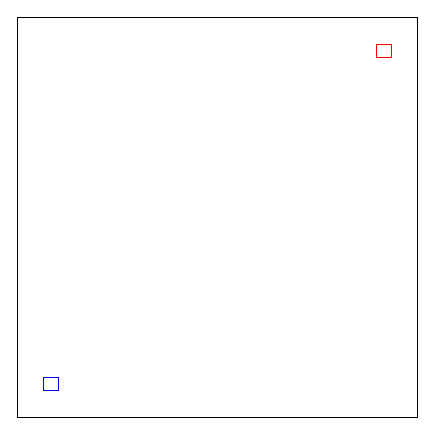
\includegraphics[width=4cm]{map.png} 
\caption{Resultado de ejemplo archivo mapa \reflistings{lst:map}.}
\label{fig:map}
\end{center}
\end{figure} 

\subsubsection*{\textit{Razonador Espacial}}

El razonador espacial es el encargado de construir la ruta que deberá recorrer el robot para llegar al objetivo.
En esta implementación se diseñó un razonador espacial que calcula la ruta óptima mediante 3 etapas \refpfigure{fig:razonador-espacial}.

\begin{figure}[H]
\begin{center}
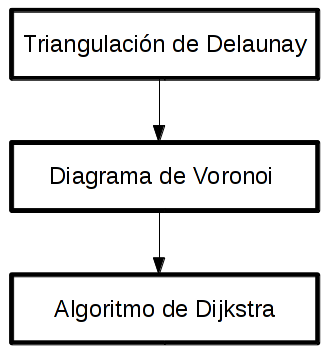
\includegraphics[width=4cm]{razonador-espacial.png} 
\caption{Etapas del razonador espacial.}
\label{fig:razonador-espacial}
\end{center}
\end{figure}

Como se muestra en la \reffigure{fig:razonador-espacial}, en la primera etapa se realiza una segmentación del mapa
a través de la \textbf{Triangulación de Delaunay}, esto divide el espacio en secciones pequeñas y conectadas. En segundo lugar
se genera un \textbf{Diagrama de Voronoi} a partir de la triangulación, este diagrama representará el mapa
en un grafo conectado. Por último, se aplica el \textbf{Algoritmo de Dijkstra} sobre el Diagrama de Voronoi con el fin
de calcular la ruta óptima desde un punto de inicio hasta un punto objetivo dentro del grafo.


\begin{enumerate}
\item \textbf{Triangulación de Delaunay:}
\item \textbf{Diagrama de Voronoi:}
\item \textbf{Algoritmo de Dijkstra:} Este algoritmo fue diseñado por Edsger Dijkstra en 1959 \cite{sniedovich2006,lavalle2006,cormen2001}, se puede categorizar en la familia de algoritmos voraces y posee una complejidad de $O(n^{2})$. Tiene como objetivo hayar todos los caminos con costo mínimo desde un nodo inicial a todos los demas nodos dentro de un grafo ponderado. Basicamente lo que hace este algoritmo es recorrer los nodos adyacentes a un nodo especifico, si encuentra un nodo con un alguna alternativa más óptima
actualiza su peso y le indica cual es su nuevo nodo ancestro .

Se explicara el algoritmo a través de su pseudocódigo (Algoritmo \ref{alg:dijkstra}).
Se tienen los siguietes elementos:

\begin{itemize}
\item $G$: el grafo
\item $Q$: cola de prioridad
\item $s$: nodo inicial
\end{itemize}

Se inicializan todos los pesos acumulados de los nodos en infinito y todos los nodos ancestros en nulo. 
Luego se agrega el nodo inicial a la cola de prioridad. 
Se procede a recorrer la cola de prioridad, mientras esta sea distinta de vacio se toma el primer elemento. 
Posteriormente se verifica el peso acumulado de cada nodo adyacente al primer elemento en la cola, si el peso acumulado del nodo actual del ciclo es mayor
al peso del primer elemento ($u$) más el peso entre ambos nodos, se actualiza el peso acumulado y el nodo ancestro del nodo actual.
Por último se agrega a la cola de prioridad el nodo adyacente. 

\begin{algorithm}
\DontPrintSemicolon
\KwData{Nodo inicial $s$}
\KwResult{Ruta óptima}

Inicializar $Q$ y $G$\;

\For{$u~\epsilon~G.getNodos()$}{
 u.setPesoAcumulado(INFINITO)\;
 u.setNodoAncestro(NULL)\;
}

s.setPesoAcumulado(0)\;
Q.adicionar(s)\;

\While{$Q\neq\emptyset$}{
	u = Q.getPrimero()\;
	\For{$v~\epsilon~u.getNodosAdyacentes()$}{ 
		\If{v.getPesoAcumulado() > u.getPesoAcumulado() + G.getPesoEntreNodos(u,v)}{
			v.setPesoAcumulado(u.getPesoAcumulado() + G.getPesoEntreNodos(u,v))\;
			v.setNodoAncestro(u)\;
			Q.adicionar(v)\;
		}
	}
}

\caption{Algoritmo de Dijkstra \label{alg:dijkstra}}
\end{algorithm}


\end{enumerate}

\subsubsection*{\textit{Secuenciador del Plan}}

\subsection*{Capa Reactiva}

\pagebreak
\section*{Herramienta de Software Desarrollada}

Se desarrolló una herramienta computacional llamada \textbf{AriaJavaP3DX}, que provee los elementos gráficos necesarios para 
configurar y monitorear el comportamiento del robot Pioneer P3DX.

Como se muestra en las Figuras \ref{fig:ventana-principal-partes} y \ref{fig:ventana-principal2}, la ventana principal está compuesta por 8 elementos básicos:

\begin{figure}[H]
\begin{center}
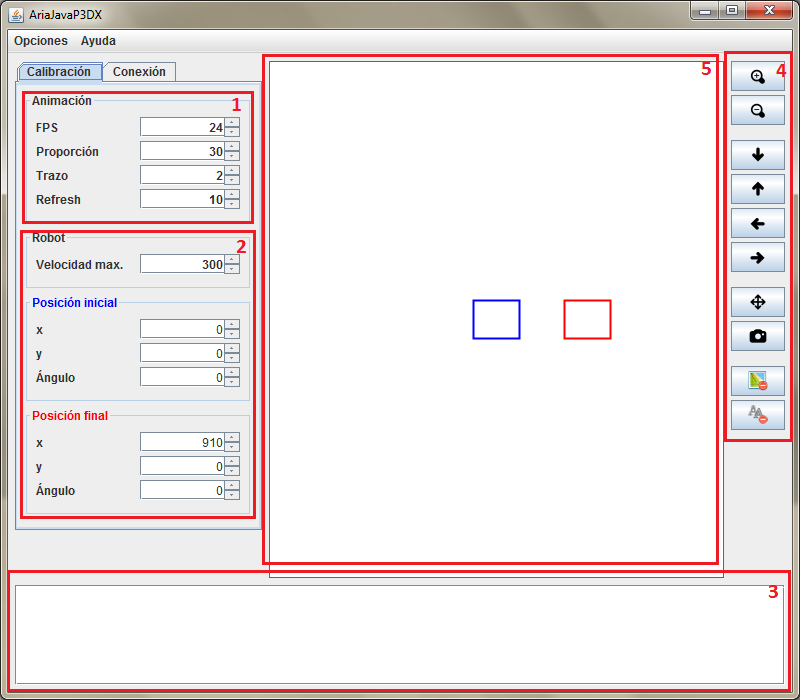
\includegraphics[width=10cm]{ventana-principal-partes.png} 
\caption{Partes de la ventana principal.}
\label{fig:ventana-principal-partes}
\end{center}
\end{figure}

\begin{figure}[H]
\begin{center}
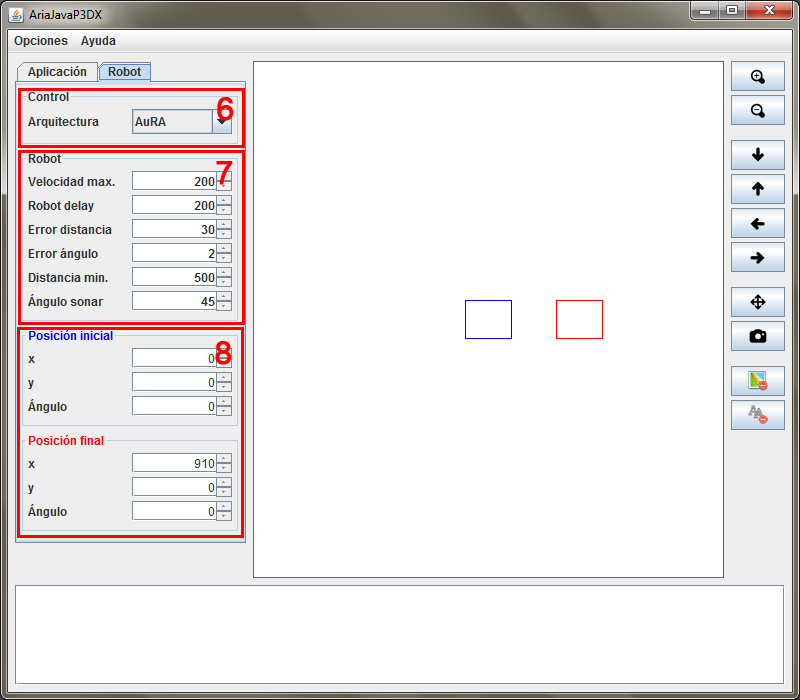
\includegraphics[width=10cm]{ventana-principal2-partes.png} 
\caption{Partes de la ventana principal.}
\label{fig:ventana-principal2}
\end{center}
\end{figure} 

\begin{enumerate}
\item Esta sección permite configurar la animación 
a través de los siguientes items: \textbf{FPS}, cuadros por segundo (en ingles \comillas{Frames per second}), 
se refiere a la frecuencia en que se actualiza la imagen de la animación. \textbf{Proporción}, es la proporción del mapa en 
la animación con respecto a la medida original en milímetros. \textbf{Trazo}, es el grosor del trazado de las imágenes en la 
animación. \textbf{Sincronización}, es la frecuencia en segundos en que se verifica la posición real del robot y se actualiza la 
posición del robot animado.
\item En el panel \textbf{Conexión} se establece la dirección IP y el puerto de conexión con el robot.
\item En la región central de la ventana se localiza la animación, se puede observar un ejemplo en la \reffigure{fig:mapa-cargado}. 
\item En el lateral derecho de la ventana se encuentran una serie de botones que permiten manipular el mapa.
 En primer lugar 
se puede hacer zoom sobre el mapa \refpfigure{subfig:botones-zoom}. Además se puede mover la ubicación del mapa hacia los 4 puntos 
cardinales \refpfigure{subfig:botones-mover-mapa}. Por otra parte, se puede centrar el mapa \refpfigure{subfig:botones-centrar-capturar} y hacer una captura de imagen, al presionar el botón de captura de imagen (ícono cámara fotográfica) se
muestra la ventana de guardar imagen \refpfigure{fig:guardar-imagen}. Los últimos botones \refpfigure{subfig:botones-ocultar-mapa} permiten mostrar u ocultar
la ruta óptima calculada y activar o desactivar el antialiasing.
\item En la parte inferior de la ventana se encuentra la consola, permite observar los mensajes que se generan en la ejecución
de la aplicación.
\item En este panel se puede establecer la arquitectura de control del robot.
En el item \textbf{Arquitectura}, se puede elegir entre la arquitectura AuRA o un comportamiento solamente reactivo.
\item Este panel permite manipular el conjunto de variables que permiten calibrar el comportamiento del robot, estas son:
\begin{enumerate}
\item \textbf{Velocidad max.:} velocidad máxima alcanzada por el robot.
\item \textbf{Robot delay:} tiempo de espera entre acciones.
\item \textbf{Error distancia:} distancia máxima permitida entre el robot y los objetivos.
\item \textbf{Error ángulo:} diferencia máxima permitida entre el ángulo del robot y el ángulo deseado.
\item \textbf{Distancia min:} distancia mínima tolerada entre el robot y un obstáculo.
\item \textbf{Ángulo sonar:} rango de detección del sonar.
\end{enumerate}
\item Esta última sección esta destinada a asignar la posición de inicio y fin del robot.
\end{enumerate} 

\begin{figure}[H]
        \centering
        \begin{subfigure}[b]{0.2\linewidth}
        		\centering
                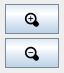
\includegraphics[width=1cm]{botones-zoom.png}
                \caption{Zoom}
                \label{subfig:botones-zoom}
        \end{subfigure}
        ~ 
        \begin{subfigure}[b]{0.2\linewidth}
        		\centering
                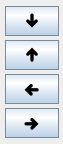
\includegraphics[width=1cm]{botones-mover-mapa.png}
                \caption{Mover}
                \label{subfig:botones-mover-mapa}
        \end{subfigure}
        ~ 
        \begin{subfigure}[b]{0.2\linewidth}
        		\centering
                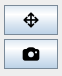
\includegraphics[width=1cm]{botones-centrar-capturar.png}
                \caption{Capturar}
                \label{subfig:botones-centrar-capturar}
        \end{subfigure}
        ~ 
        \begin{subfigure}[b]{0.2\linewidth}
        		\centering
                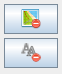
\includegraphics[width=1cm]{botones-ocultar-mapa.png}
                \caption{Ocultar}
                \label{subfig:botones-ocultar-mapa}
        \end{subfigure}
        \caption{Acciones para manipulación del mapa.}
        \label{fig:botones-mapa}
\end{figure}

\begin{figure}[H]
\begin{center}
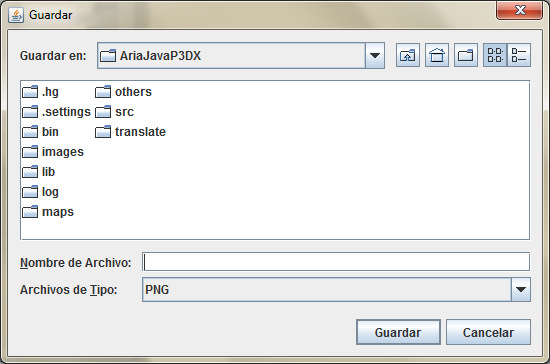
\includegraphics[width=6cm]{guardar-imagen.png} 
\caption{Ventana para guardar captura del mapa.}
\label{fig:guardar-imagen}
\end{center}
\end{figure} 

\begin{figure}[H]
\begin{center}
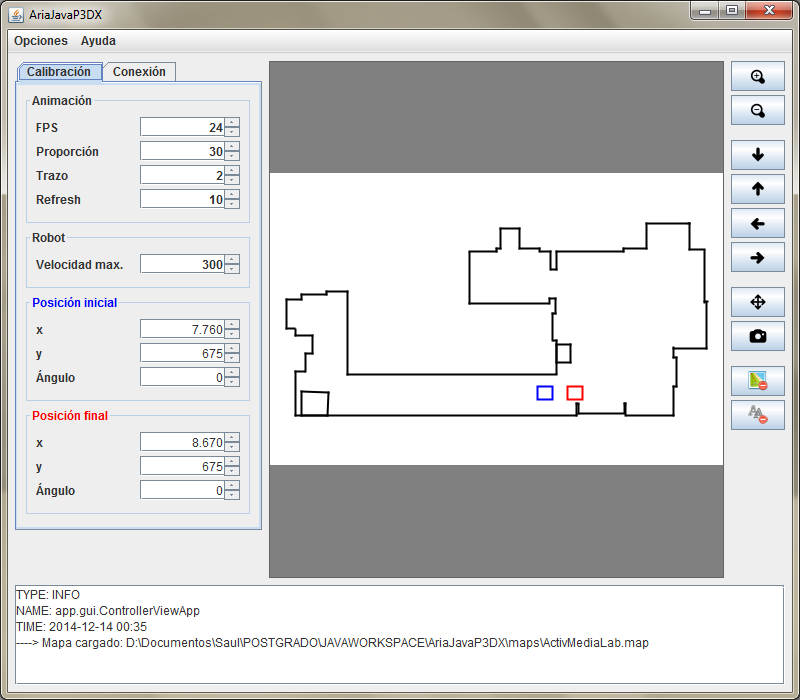
\includegraphics[width=10cm]{mapa-cargado.png} 
\caption{Mapa cargado.}
\label{fig:mapa-cargado}
\end{center}
\end{figure} 

\pagebreak
\subsubsection*{\textit{Menú Opciones}}

A través de este menú \refpfigure{fig:menu-opciones} se puede seleccionar y cargar un mapa ingresando 
a la opción \textbf{Cargar Mapa}, esta, desplegará una ventana de búsqueda \refpfigure{fig:cargar-mapa}.
La opción \textbf{Ver configuración} permite visualizar la lista de valores de la configuración general de la aplicación \refpfigure{fig:ver-configuracion}. Por último la opción cerrar permite terminar la aplicación.

\begin{figure}[H]
\begin{center}
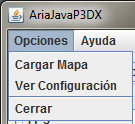
\includegraphics[width=2cm]{menu-opciones2.png} 
\caption{Menú opciones.}
\label{fig:menu-opciones}
\end{center}
\end{figure} 

\begin{figure}[H]
\begin{center}
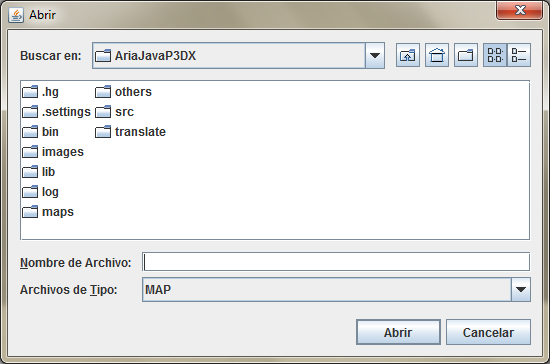
\includegraphics[width=6cm]{cargar-mapa.png} 
\caption{Ventana para seleccionar mapa.}
\label{fig:cargar-mapa}
\end{center}
\end{figure} 

\begin{figure}[H]
\begin{center}
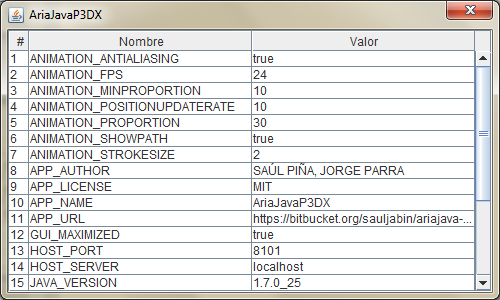
\includegraphics[width=6cm]{ver-configuracion.png} 
\caption{Ventana para ver los atributos de configuración.}
\label{fig:ver-configuracion}
\end{center}
\end{figure} 

\subsubsection*{\textit{Menú Ayuda}}

A través del menu ayuda \refpfigure{fig:menu-ayuda} se puede acceder a la documentación de 
la aplicación, además se puede ingresar a la ventana de creditos en la opción \textbf{Sobre AriaJavaP3DX} \refpfigure{fig:ventana-about}.

\begin{figure}[H]
\begin{center}
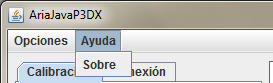
\includegraphics[width=3cm]{menu-ayuda2.png} 
\caption{Menu Ayuda.}
\label{fig:menu-ayuda}
\end{center}
\end{figure} 

\begin{figure}[H]
\begin{center}
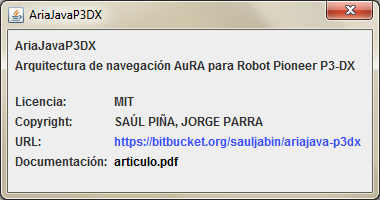
\includegraphics[width=6cm]{ventana-about.png} 
\caption{Ventana para ver la información de la aplicación.}
\label{fig:ventana-about}
\end{center}
\end{figure} 

\section*{Experimentación}

\section*{Conclusión}

%%%%%%%%%%%%%%%%%%%%%%%%%%%%%%%%%%%%%%%%%%%%%%%%%%%%%%%%%%%%%%%%%%%%%%%%%%%%%%%%%%%%%%%%
%                                 BIBLIOGRAFIA
%%%%%%%%%%%%%%%%%%%%%%%%%%%%%%%%%%%%%%%%%%%%%%%%%%%%%%%%%%%%%%%%%%%%%%%%%%%%%%%%%%%%%%%%
\begin{thebibliography}{999}

\bibitem{arkin1997}
	Arkin, R. y Balch, T. (1997).
 	AuRA: Principles and practice in review.
	Journal of Experimental \& Theoretical Artificial Intelligence.
	Taylor \& Francis. Vol. 9. No. 2-3. Pp. 175-189.
	
\bibitem{aria2014} 
	MobileRobots. (2014).
	ARIA. 	
	Disponible en: \\\link{http://robots.mobilerobots.com/wiki/ARIA}.
	
\bibitem{mobilesim2014} 
	MobileRobots. (2014).
	MobileSim. 	
	Disponible en: \\\link{http://robots.mobilerobots.com/wiki/MobileSim}.
	
\bibitem{eclipse2014} 
	Eclipse. (2014).
	Eclipse IDE. 	
	Disponible en: \\\link{https://www.eclipse.org/ide/}.

\bibitem{java2014} 
	Oracle. (2014).
	Java. 	
	Disponible en: \\\link{http://www.oracle.com/technetwork/java/index.html}.
	
\bibitem{mapper2014} 
	MobileRobots. (2014).
	Mapper3. 	
	Disponible en: \\\link{http://robots.mobilerobots.com/wiki/Mapper3}.
	
\bibitem{sniedovich2006} 
	Sniedovich, M. (2006). 
	Dijkstra's algorithm revisited: the dynamic programming connexion. 
	Control and cybernetics.
	Vol. 35. No. 3. Pp. 599-620.

\bibitem{lavalle2006} 
	Lavalle, S. (2006). Planning algorithms. Cambridge university press.
	
\bibitem{cormen2001} 
	Cormen, T., Leiserson, C., Rivest, R., y Stein, C. (2001). Introduction to algorithms. Cambridge: MIT press.
	
\end{thebibliography}
\end{document}
